\chapter{Анализ средств сборки и визуализации программного обеспечения} \label{ch1}

% не рекомендуется использовать отдельную section <<введение>> после лета 2020 года
%\section{Введение. Сложносоставное название первого параграфа первой главы для~демонстрации переноса слов в содержании} \label{ch1:intro}

В первой главе рассмотрим:

\begin{enumerate}
	\item Процесс и инструменты сборки приложения.
	
	\item Анализ средств сборки программного обеспечения%%Анализ средств ??? %%CI/CD в контексте сборок приложения.
	
	\item Понятие статистик и визуализации сборок в контексте инструментов CI/CD.
	
	\item Обзор и сравнительный анализ плагинов Jenkins по визуализации статистики работы сборок.
	
	\item Требования к разработке.
	
	
\end{enumerate}

\section{Анализ средств сборки программного обеспечения} \label{ch1:sec1}

Для осуществления сборки программного продукта существует множество инструментов, какое средство использовать определяют не только из преимуществ и недостатков этих средств, но и исходя из того, какой используется язык программирования, фреймворк и окружение.
На данный момент существует большое количество инструментов сборки приложения. 

Maven — инструмент для автоматизации сборки проектов, который используется с Java приложениями. Maven решает несколько проблем \cite{maven}:

\begin{itemize}
	\item  упрощение процесса сборки;
	\item обеспечение единой системы сборки;
	\item предоставление информации о проекте;
	\item упрощение работы с зависимостями, включая их автоматическое обновление.
\end{itemize}

Gradle — система автоматизации сборки, которая также часто используется для Java разработки. Gradle включает в себя следующие возможности \cite{gradle}:

\begin{itemize}
	\item декларативное описание сборки;
	\item управление зависимостями;
	\item создание многомодульных проектов;
	\item плагины.
\end{itemize}

Для проектов на JavaScript для управления зависимостями и сборками может использоваться npm в связке с Webpack. Webpack это инструмент для сборки и оптимизации приложений Node.js. Преимущества инструмента  \cite{webpack}:

\begin{itemize}
	\item разбивки пакетов на мелкие фрагменты;
	\item поддержка плагинов;
	\item большое сообщество.
\end{itemize}

Также данный сборщик обладает такими недостатками, как высокий порог вхождения и низкая скорость сборки.

Также необходимо отметить, что в отличии от компилируемых языков, таких как Java, приложения на интерпретируемом языке Python могут запускаться без сборки прямо из командной строки, а для управления зависимостями в Python используется инструмент pip.

Существуют также и другие инструменты сборки для приложений написанных на разных языках программирования. Все их удобно использовать при локальной разработке над небольшими проектами, но когда рассматривается вопрос о разработке большого продукта, в работе над которым задействуется целая команда разработчиков и тестировщиков, для уменьшения затрат на разработку, в первую очередь временных, следует внедрять DevOps практики и CI/CD подходы.

Инструменты CI/CD позволят взаимодействовать с репозиторием гита, проводить сборку продукта автоматически по заданному времени или по наличию новых коммитов, прогонять тесты после каждого изменения разработчика, производить установку на различные стенды, а также выполнять сборку различных компонентов системы одновременно и доставлять продукт заказчику. Перейдем к рассмотрению особенностей CI/CD инструментов, а затем рассмотрим сравнение их между собой.


\section{Анализ средств CI/CD} \label{ch1:sec3}

%\subsection{Особенности CI/CD систем} \label{ch1:sec2}%и сравнительный анализ PA: сравнительный анализ здесь отсутствует.

CI/CD — это технология автоматизации тестирования и доставки/развертывания готового приложения заказчику  \cite{cicd}. Данная технология стала неотъемлемой составляющей DevOps методологии и помогает сократить временные  ресурсные затраты в процессе современного жизненного цикла приложения, когда до заказчика изначально доходит минимально жизнеспособный продукт (MVP), а затем дорабатывается с учетом новых требований заказчика, т.е. идет непрерывная разработка новых версий продукта.

Преимущества CI/CD подхода \cite{plusci}:

\begin{itemize}
	\item упрощение разработки - позволяет разработчикам распределять приоритеты и сконцентрироваться на самых важных аспектах;
	\item улучшение качества кода -  качество кода проверяется до того, как он достигнет среды тестирования, проблемы в коде могут быть выявлены на ранних стадиях;
	\item более короткие циклы тестирования - меньший объем кода для проверки, становиться проще определить проблемы в процессе развертывания;
	\item более простой мониторинг изменений - меньший объем кода для проверки;
	\item более легкий откат - меньшие усилия для отката приложения к предыдущей версии при возникновении проблем в новой версии.
\end{itemize}

Этапы разработки и принцип CI/CD подхода можно отразить с помощью рисунка 1.

\begin{figure}[ht!] 
	\center
	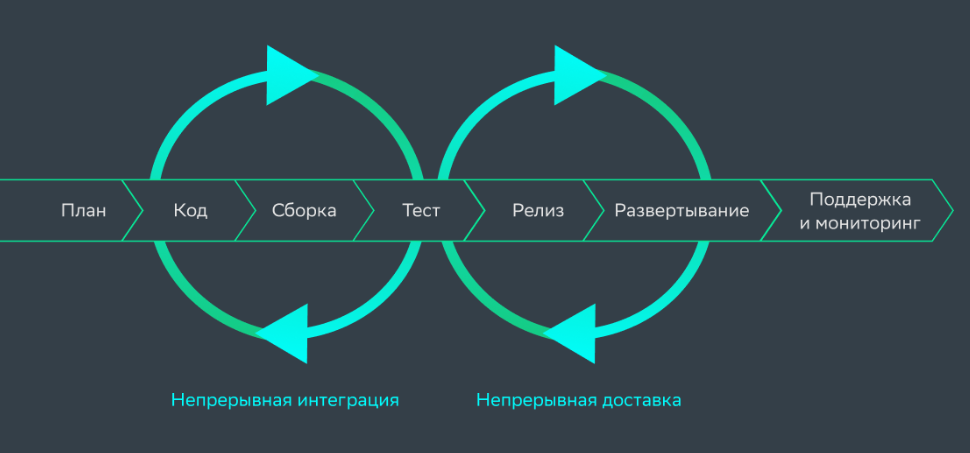
\includegraphics [scale=0.67] {my_folder/images//cicdalter}
	\caption{Цикл CI/CD \cite{cycleci}} 
	\label{fig:ci-cd}  
\end{figure}



На данный момент существует множеств инструментов CI/CD, которые обладают своими преимуществами и недостатками, были выделены самые распространенные системы:

\begin{itemize}
	\item TeamCity;
	\item Jenkins;
	\item GitLab CI;
	\item CircleCI;
	\item Bamboo.
\end{itemize}




Jenkins — это автономный сервер автоматизации с открытым исходным кодом, который можно использовать для автоматизации всех видов задач, связанных со сборкой, тестированием, доставкой или развертыванием программного обеспечения \cite{jenkins}.

TeamCity - это сервер CI от компании Jetbrains  \cite{tc}, который позволяет запускать параллельные сборки одновременно на разных платформах и средах, а также настраивать статистику по продолжительности сборки, уровню успешности, качеству кода и пользовательским метрикам.

GitLab CI - сервер CI от компании GitLab \cite{gitlab}, которая также предоставляет одноименный репозиторий Git. GitLab CI/CD может обнаруживать ошибки на ранних этапах цикла разработки и гарантировать, что весь код, развернутый в рабочей среде, соответствует установленным стандартам кода.

CircleCI - сервер CI \cite{circle}, который позволяет настроить для эффективной работы очень сложных конвейеров кэширование, кэширование уровня Docker и классы ресурсов для работы на более быстрых машинах.

Bamboo — это инструмент непрерывной интеграции и доставки  \cite{bamboo}, который связывает автоматизированные сборки, тесты и выпуски в единый рабочий процесс.

В таблице 1.1 указан, краткий сравнительный анализ плагинов. Стоит сразу отметить, что \textit{сравнение платных и бесплатных решений не корректно}, поскольку организации, которые выпускают коммерческие продукты обладают куда большими возможностями в сравнении с компаниями, которые не берут плату за использование своего продукта. Что наглядно видно из сравнительного анализа Jenkins с остальными средствами CI.

Особое внимание следует уделить критерию OpenSource, этот критерий является достаточно важным с учетом, того, что многие компании после 2022 года ушли из РФ, тем самым стали либо недоступны, либо прекратили лицензировании и стали менее безопасными, т.к. новые версии продуктов больше недоступны и проблемы с безопасностью и другими дефектами не будут исправлены/доступны на территории РФ. Также критерий важен тем, что даже при наличии действия продуктов компаний, они обходилось крупным ИТ-компаниям достаточно дорого.

\begin{table}
    \centering
    \caption{Сравнительный анализ инструментов CI/CD}
    \begin{tabular}{|p{3cm}|p{2cm}|p{2cm}|p{2cm}|p{2cm}|p{2cm}|}
    \hline
        Критерий & Jenkins & TeamCity & GitLab CI & CircleCI & Bamboo \\ \hline
        Открытый исходный код & + & - & + & - & - \\ \hline
        Цена & Бесплатно & от 45\$ в месяц \cite{cianalyze} & от 21\$ в месяц \cite{gitlabprice} & от 15\$ в месяц \cite{cianalyze} & от 1200\$ в год \cite{cianalyze} \\ \hline
        Поддержка вендора & - & + & + &+ & + \\ \hline
        Поддержка репозиториев Git & Любой репозиторий & GitHub, GitLab, Bitbucket & GitHub, GitLab, Bitbucket  & GitHub, GitLab, Bitbucket & Любой репозиторий  \\ \hline

    \end{tabular}
\end{table}	

Также необходимо отметить еще 2 критерия для более объективной оценки: интеграции - количество интеграций инструмента со сторонними средствами и встроенная функциональность - количество встроенных функций.
Критерий интеграция показывает сколько можно подключить к системе плагинов и интеграций со сторонними сервисами, а встроенный функционал сколько функций из коробки поддерживает, то или иное средство, наличие инструментов, которые позволят облегчить работу.

Если сравнивать описанные выше средства, то TeamCity обладает самой мощной встроенной функциональностью, а также достаточно большим количеством интеграций и плагинов \cite{cianalyze}, в сравнении со всеми остальными инструментами, за исключением Jenkins.

Jenkins в отличие от перечисленных коммерческих средств обладает самой низкой встроенной функциональностью, также отсутствует возможность построения конвейеров, но при этом все эти недостатки закрываются большим количеством плагинов, которые постоянно пишутся разработчиками, среди плагинов имеется и pipeline, который и нужен для построения конвейеров, количество плагинов около 2 тысяч, что в несколько раз больше, чем у TeamCity, в котором около 500 плагинов и интеграций.

Среди всех средств особо ярко выделяется Jenkins, поскольку он является бесплатным и с открытым исходным кодом, а также обладает большим количество интеграций и плагинов, которые постоянно пишутся, что позволяет устранить основной его недостаток по наличию встроенных функций. После 2022 года в РФ это стал самый востребованный инструмент для настройки CI конвейеров, и обосновывает важность разработки плагина для устранения недостатков функциональности, которые есть в других средствах.
 
 
\section{Анализ существующих плагинов Jenkins по визуализации статистики сборок} \label{ch1:sec5}


% \section{Статистика и визуализация работы сборок в контексте CI/CD} \label{ch1:sec4}

Поскольку для работы со сборками приложений был выбран Jenkins, то разработка плагина будет производиться в этой системе. В любой системе с большим количеством приложений, сборок и тестов будет удобно производить мониторинг и визуализацию информации по статистике работы сборок во времени. 

Под статистикой работы сборок будем понимать следующие статистические характеристики собираемых метрик (продолжительность исполнения сборки, время проведенное в очереди сборкой, размеры полученных по итогам сборки артефактов):

\begin{itemize}
	\item среднее арифметическое;
	\item мода;
	\item медиана;
	\item размах;
	\item среднеквадратическое отклонение;
	\item среднеквадратическое отклонение несмещенное;
	\item дисперсия.
\end{itemize}

% ВОДА СОКРАТИТЬ???
% В данной работе производится разработка плагина для визуализации метрик сборки Jenkins, основанием для разработки является отсутствие плагина, который полностью визуализирует метрики сборок в Jenkins, аналогично  %встроенному модулю в TeamCity. Многие российские ИТ-компании использовали TeamCity, этот модуль позволял отслеживать состояние отдельных конфигураций сборки с течением времени,собирать статистические данные по всей  %истории сборки и отображать их в виде наглядных диаграмм. В данной работе будет разработан плагин для воссоздания этого модуля в Jenkins, с дополнительным функционалом, которого не хватало в TeamCity.

В данной работе будет разработан плагин для воссоздания модуля Statistics в Jenkins, с дополнительным функционалом, которого не хватало в TeamCity, который позволял отслеживать состояние отдельных конфигураций сборки с течением времени, собирать статистические данные по всей истории отдельного задания и отображать их в виде наглядных диаграмм.

Для оценки плагинов, необходимо понять какие метрики требуется для сбора статистики работы сборок. Требуется реализовать следующие метрики:

\begin{itemize}
	\item визуализация метрики success rate (SR) - процент успешности сборок, который будет показывать сколько сборок завершилось успешно;
	\item визуализация метрики Build Duration (BD) - время выполнения сборок, в том числе должен быть доступен фильтр на добавления в график упавших сборок, а также возможность вычислять не только суммарно время сборок, а также среднее время всех сборок за определенный интервал времени;
	\item визуализация метрики Time Spent in queue (TQ) - время проведенное в очереди сборок, в том числе среднее время, вычисляемое аналогично Build Duration;
	\item  визуализация метрики Test Count (TC) - количество выполненных тестов в сборке, в том числе количество выполненных тестов в упавших сборках, если таковые успели выполниться;
	\item визуализация метрики Artifacts Size (AS) - размер созданных во время сборок артефактов, в том числе средний размер за определенный интервал времени, а также учет артефактов, которые успели создаться в сборках до падения.
\end{itemize}

Сначала рассмотрим уже разработанные плагины визуализации и их недостатки и преимущества в сравнении с разрабатываемым решением. Результаты сравнения приведены в таблице 1.2.

\begin{table}
    \centering
    \caption{Сравнительный анализ плагинов Jenkins}
    \begin{tabular}{|p{5cm}|p{2cm}|p{3cm}|p{3cm}|p{2cm}|}
    \hline
        Критерий & Build Monitor Plugin \cite{buildmonitor} & Global Build Stats Plugin \cite{gstats} & Build Time Blame \cite{buildblame} & Плагин разрабатываемый  \\ \hline
        Прогнозирование метрик следующей сборки  & - & - & - & +  \\ \hline
        Открытый исходный код  & + &+ & + & +  \\ \hline
        Визуализация времени выполнения и статуса последней сборки & + &+ & - (только время) &+  \\ \hline
        Визуализация SR истории сборок & - & +/- (в TeamCity гистограммы, которые показывают процентное соотношение нагляднее) & - & +  \\ \hline
       Визуализация BD истории сборок (в числе average) & - & + & +  & +  \\ \hline
       Визуализация TQ & - & - & -  &+  \\ \hline
      Визуализация TC & - & - & +  & +  \\ \hline
      Визуализация AS & - &- &-  & +  \\ \hline
       Отображение всех графиков на одной странице по одному диапазону времени для наглядного отображения всех метрик в один момент и во времени & - & + & -  & +  \\ \hline


    \end{tabular}
\end{table}	

 Build Monitor Plugin - плагин, который обеспечивает наглядное представление статуса выбранных заданий Jenkins. Отображает состояние и ход выполнения выбранных заданий \cite{buildmonitor}.
 
 Global Build Stats Plugin - плагин, который позволит собирать и отображать глобальную статистику результатов сборки, а также позволяющий отображать глобальную тенденцию сборки Jenkins/Hudson с течением времени  \cite{gstats}.
 
  Build Time Blame - плагин, который сканирует вывод консоли на наличие успешных сборок и генерирует отчет, показывающий, как эти шаги повлияли на общее время сборки. Это предназначено для того, чтобы помочь проанализировать, какие этапы процесса сборки являются подходящими кандидатами на оптимизацию  \cite{buildblame}.
  
  После проведения сравнения аналогичных решений, были выявлены преимущества разрабатываемого плагина, которые обосновывают его разработку, это отсутствие у данных плагинов функционала по визуализации Artifacts Size, Time Spent in queue, Success Rate истории сборок, а также наличие прогнозирования метрик следующей сборки. Также данные плагины не предлагают динамическое изменение графиков по мере изменения временного интервала или установления фильтров.



\section{Требования к разработке} \label{ch1:sec6}

Поскольку разрабатываемый плагин является аналогом модуля статистики сборок в TeamCity (поскольку TeamCity является лучшим из коммерческих инструментов и имеет удобный модуль визуализации статистики), то функционал должен как минимум реализовывать функции модуля Statistics в TeamCity. В первую очередь должна производиться визуализация метрик сборок с помощью графиков и диаграмм.

На всех графиках и диаграммах должна быть возможность выбора значения из выпадающего списка интервала времени, за который будет производиться сбор статистики за день, месяц, квартал, неделю, год.

\textit{Например}, был выбран промежуток времени месяц, то должен выполняться следующий набор действий:

\begin{enumerate}
	\item Должна собираться информация о требуемой метрики у всех сборок.
	
	\item Производиться фильтрация сборок т.е. должны отбираться только сборки за последний месяц (в том числе упавшие, если был выбран данный чекбокс).
	
	\item Полученные сборки должны группироваться по дням т.е. на итоговом графике должно быть 30/31 точка или столбца.
	
	\item Если необходимо производиться вычисление статистической обработки среди всех сгруппированных за день метрик сборок.
	
	\item Отображение всей информации о метриках сборки на одном графике или диаграмме.
	
	
\end{enumerate}

Также все графики должны располагаться друг под другом на одной странице, что может наглядно показать (если на каждом графике был выбран один период), все вычисленные метрики за один период, например при выборе месяца все перечисленные метрики будут отображены на странице и можно будет увидеть, что происходило, например вчера по результатам запуска всех сборок.

На метрикам BD, AS, TQ должна быть возможность выбрать статистический показатель, в соответствии с которым должна производить обработка итоговых значений. Возможные показатели перечислены в разделе 1.4.

Помимо прочего требуется, чтобы при визуализации можно было выбрать различные типы диаграмм: столбчатые, линейные тренды, круговые.

Также было принято решения добавить анализ данных, чтобы делать предположение, о том какими метриками будет обладать следующая запущенная сборка, при вычислении данного значения должно быть рассчитаны веса каждой сборки/сборок по графику за определенный период, и если сборка была собрана, например, месяц назад - она должна иметь меньший вес, чем сборка, собранная вчера.

Также к разработке будет предъявлено требование об удобстве интерфейса: все графики должны быть удобными, не перегруженными информацией, а также интерфейс должен быть интуитивно понятно, чтобы данный плагин не усложнял восприятие собранной статистики сборок и не вызывал желание воспользоваться другим плагином или разработать другой более удобной, или отказаться от идеи смотреть статистику по сборкам.

\section{Выводы} \label{ch1:sec7}

По всем описанным выше разделам можно прийти к выводу, что данный плагин актуален для ИТ-компаний, которые ранее отдавали предпочтению многофункциональному инструменту TeamCity, в котором уже были все необходимые для работы функции, особенно это актуально для компаний в РФ, но также может понадобиться и другим компания, которые приняли решение отказаться от TeamCity в пользу Jenkins из-за больших денежных затрат на лицензию. Также будет реализованы дополнительный функционал по сравнению с модулем TeamCity, что даст преимущества не только в цене. После проведенного обзора аналогичных решений становится понятно, что сейчас в Jenkins нет полнофункциональной замены модуля статистики TeamCity, также необходимо учесть и визуальную составляющую, чтобы при установке данного плагина разработчики выбирали его не только из-за отсутствия другого решения.













%
%

%
%
%\begin{table} [htbp]% Пример оформления таблицы
%	\centering\small
%	\caption{Представление данных для сквозного примера по ВКР \cite{Peskov2004}}%
%	\label{tab:ToyCompare}		
%		\begin{tabular}{|l|l|l|l|l|l|}
%			\hline
%			$G$&$m_1$&$m_2$&$m_3$&$m_4$&$K$\\
%			\hline
%			$g_1$&0&1&1&0&1\\ \hline
%			$g_2$&1&2&0&1&1\\ \hline
%			$g_3$&0&1&0&1&1\\ \hline
%			$g_4$&1&2&1&0&2\\ \hline
%			$g_5$&1&1&0&1&2\\ \hline
%			$g_6$&1&1&1&2&2\\ \hline		
%		\end{tabular}	
%	\normalsize% возвращаем шрифт к нормальному
%\end{table}


% \firef{} от figure reference
% \taref{} от table reference
% \eqref{} от equation reference




